\documentclass[../598comp.tex]{subfiles}

\date{05-12}

\begin{document}

\section{05-12}

\subsection{Basic Propositional Logic}

Lot's of confusion about what is meant by a true statement vs valid statement vs theorem.

\subsubsection{Syntax}
PROP = $\{p, q, r, \cdots\}$ are propositional variables.

$\varphi, \psi$ are meta-variables for describing generic propositional formulas.

Formulas are defined inductively. Inductive because you have some formulas and
you give rules for building new formulas from old ones.

This is syntax. What I'm allowed to write, but explaining anything about what
they mean. Explaining what they mean is called semantics.
\begin{enumerate}
\item 
  $T$ for true is a formula, and $\perp$ for false is a forumla.
\item
  Any propositional variable is a formula
\item
  If $\varphi$ is a formula, so is $\neg \phi$.
\item
  If $\varphi$ and $\psi$ are formulas, so are $\varphi \wedge \psi, \ \varphi
  \vee \psi, \ \varphi \Rightarrow \psi$
\end{enumerate}

\subsubsection{Proof Theory}
How to use and manipulate formulas in deduction. Proof theory is not about being
true. It's about true.

Gamma is the set of assumptions you are making.

$\gamma \cup \{\psi\}$ but we write $\gamma, \psi$

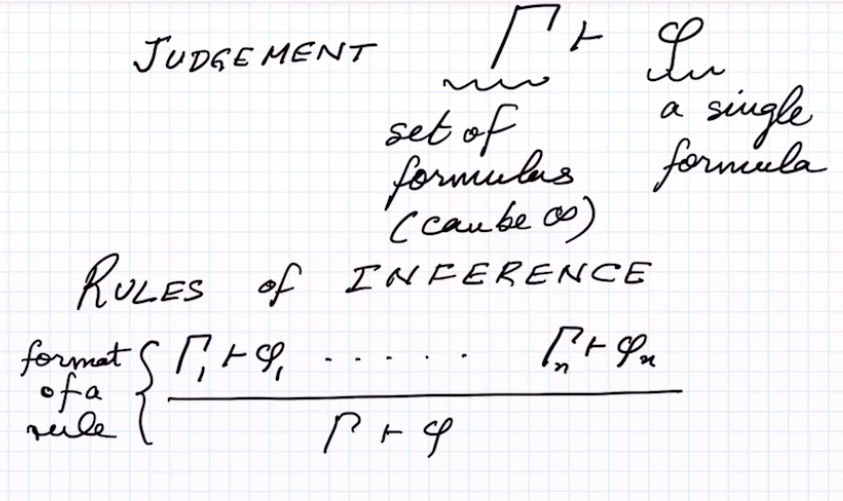
\includegraphics[width=\textwidth]{judgement_rules}
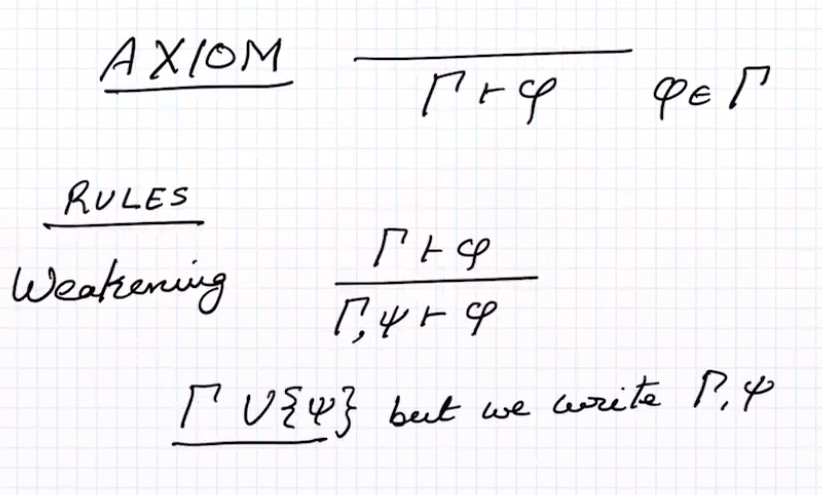
\includegraphics[width=\textwidth]{axiom_weakening}

You can do introduction or elimination.

$\neg \varphi$ is a marco for $\varphi \Rightarrow bot$.

A \ul{proof} is a tree whose leaves are axioms, the nodes are rules instances,
and the rute is a single judgement $\gamma \vdash \varphi$.

If the root has the form $\vdash$ we say that $\varphi$ is a \ul{theorem}.

\subsubsection{Semantics}
Interpret logical formulas as elements of a simple mathematical structure.
\\\\
A valuation $v: \text{PROP} \to \{0, 1\}$. Extend $v$ to a map on formulas by
structural induction.
\begin{gather*}
  v(T) = tt \quad v(\bot) = ff \\
  v(\varphi) \underbrace{\wedge}_{\text{Boolean algebra}} v(\varphi') = v(\varphi \underbrace{\wedge}_{\text{Syntax}}\varphi')
\end{gather*}

If $\models \varphi$, then $\forall v, \ v(\varphi) = tt$. Such a formula is
called a \ul{tautology}.
\\\\
$\vdash$ denotes a syntactic implication while $\models$ denotes a semantic implication.

\begin{theorem}[Soundness]
  If $\gamma \vdash \varphi$ then $\gamma \models$ in particular if $\vdash \varphi$
  then $\models \varphi$.
\end{theorem}
\begin{theorem}[Completeness]
  If $\gamma \models \varphi$ then $\gamma \vdash \varphi$.
\end{theorem}

Suppose that $\gamma$ has no valuation such that $\forall \varphi \in \gamma, \
v(\varphi) = tt$. Then we say that $\gamma$ is \ul{unsatisfiable}.

\begin{theorem}[Compactness]
  If $\gamma$ is unsatisfiable, then some \ul{finite subset} of $\gamma$ is unsatisfiable.
\end{theorem}
\begin{remark}
  Tepmoral logic fails this property.
\end{remark}

\subsection{Temporal Logic}
as opposed to propositional logic. The basic atomic properties can change their truth values in time.

A mir Puuli showed this is very useful for reasoning about code execution
especially \ul{concurrent} programs.

\subsubsection{Syntax}
PROP = $\{p, q, r, \dots\}$. Formulas $\neg, \wedge, \dots$. Two temporal
operators $O, u$. If $\varphi$ is a formula then $0\varphi$ is a formula. If
$\varphi, \psi$ are formulas, then $\varphi u \psi $ is a formula.

$\varphi = true |p| \varphi_1 \wedge \varphi_2 |\neg \varphi| O\varphi |\varphi
u \psi$

Intuition. Instead of a valuation we have a \ul{linear sequence} of valuations.
We will call these valuations states. The entire sequence is called a history.

Defined operators.
\subsection{Labelled Transition System}

$(S, Act, \to, I, AP, L)$
$S$ states perhaps infinite. $Act$ actions. $\to \subseteq S \times A \times S$.
represents function $a$ $s \to s'$
$I \subseteq S$. initial states. AP are the set of atomic propositions.
\end{document}